%%%%%%%%%%%%%%%%%%%%%%%%%%%%%%%%%%%%%%%%%%%%%%
%                insertmeeting
% 1) Title (something creative & funny?)
% 2) Date (MM/DD/YYYY)
% 3) Location (ex. Hagerty High School)
% 4) People/Committees Present 
% 5) Picture 
% 6) Start Time & Stop Time (ex. 12:30AM to 4:30PM)
%%%%%%%%%%%%%%%%%%%%%%%%%%%%%%%%%%%%%%%%%%%%%%
\insertmeeting 
  {Coopertition} 
  {01/17/22} 
  {Hagerty High School}
  {Falon, James, Jensen, Nathan, Ritam, Rose, Samantha}
  {Images/RobotPics/robot.jpg}
  {2:30 - 4:30}
  
\hhscommittee{Strategy}
\noindent\hfil\rule{\textwidth}{.4pt}\hfil
\subsubsection*{Goals}
\begin{itemize}
    \item Design and create a new team element that can be Capped by Roarbots  

\end{itemize} 

\noindent\hfil\rule{\textwidth}{.4pt}\hfil

\subsubsection*{Accomplishments}
Today, we got together to determine how we could cap during end game. We determined that at this point, it may be better to just make a team element that our alliance partner can cap. This is when we began to discuss who we would be most likely to chose if we were alliance captains and a few names came up. Firstly there was Roarbots. Roarbots is the team that we were able to beat the Florida state record. It was also helpful that they can cap so we thought it may be good to create an element that Roarbots can cap so we can double cap. Another team that was discussed was Zip Ties. Their cap is very unique in the fact that it is just a blue cylinder. This means that it would be hard to cap on top of theirs but we determined that we could possibly make a cap with a circular base that they could possibly be able to pick up. Another team that came up was our sister team Metalmorphosis (4227) they were able to cap a team element if there was a cube on the top. So we decided to create an element that was compatible with them just in case we were on the same team at any point.
To begin designing the elements, we took the dimensions of Roarbot's element. This allowed us to ensure compatibility between the mechanism and our element. Next we noticed flaws in the design. We decided to make holes at the bottom where we could put in ball bearings to weigh it down. This would shift the center of gravity closer to the ground and make it harder to flip.
The other elements were much simpler to create as we just took the Roarbot's element that we had already made and changed the base and top mounting accessory. Though we are not positive that these elements will work, we intend to have the teams that we created caps for to be at a scrimmage the day before leagues. This allows us to collaborate and determine any changes we need to make and what alliance partners we would like should we be in finals.
 

\begin{figure}[ht]
\centering
\begin{minipage}[b]{.48\textwidth}
  \centering
  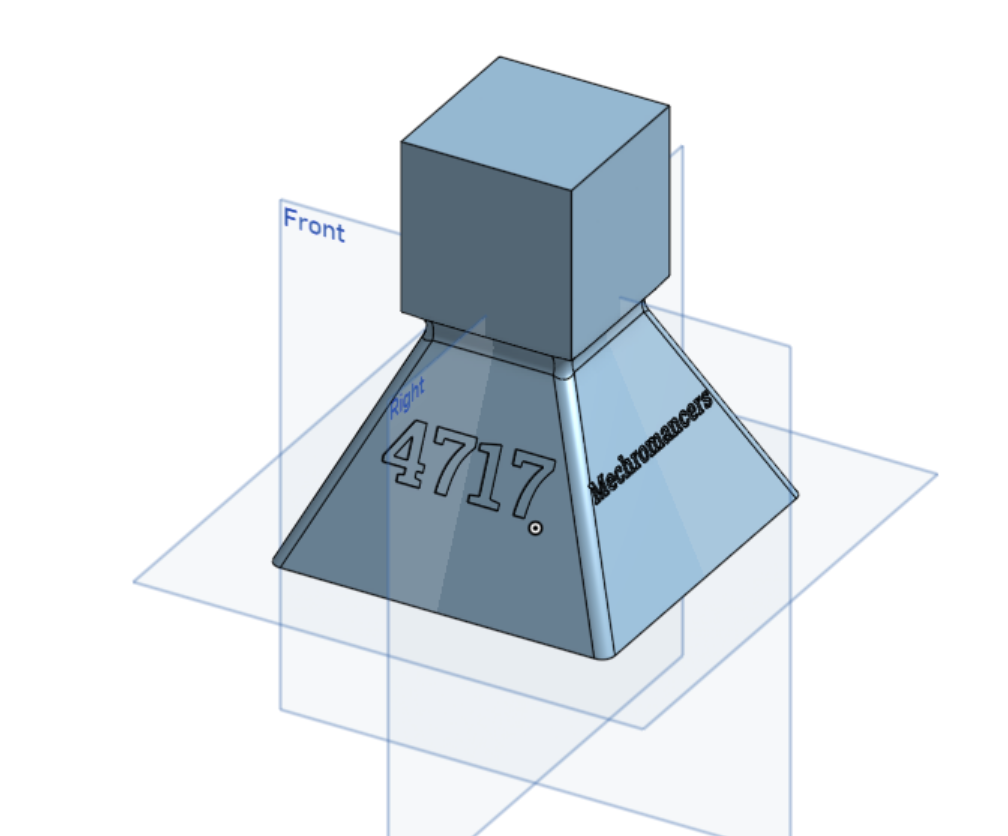
\includegraphics[width=0.95\textwidth]{Meetings/January/01-17-22/4227 Element - Jensen Miller.PNG}
  \caption{4227's game element}
  \label{fig:011722_1}
\end{minipage}%
\hfill%
\begin{minipage}[b]{.48\textwidth}
  \centering
  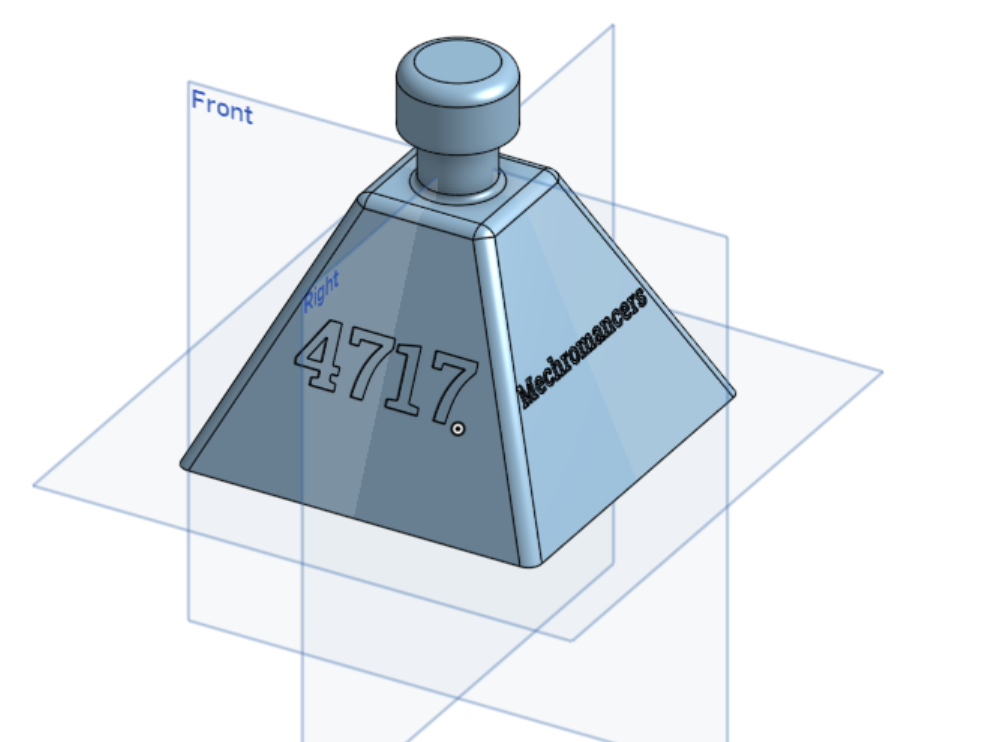
\includegraphics[width=0.95\textwidth]{Meetings/January/01-17-22/Roarbots Element - Jensen Miller.PNG}
  \caption{Roarbots's element}
  \label{fig:011722_2}
\end{minipage}
\end{figure}

\begin{figure}[htp]
\centering
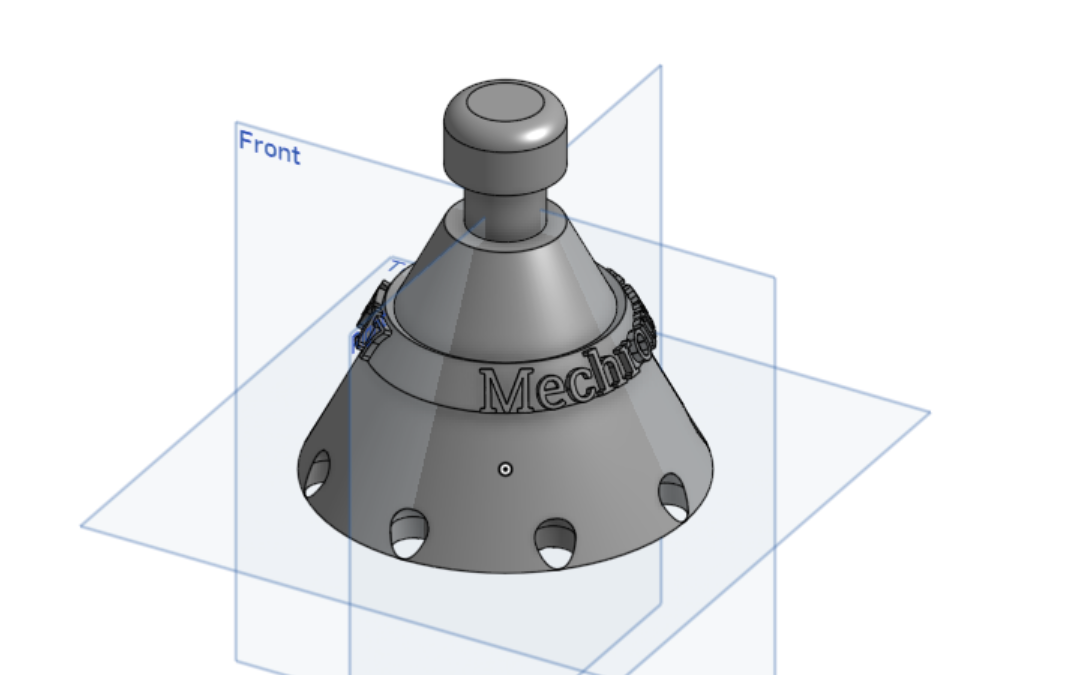
\includegraphics[width=0.95\textwidth, angle=0]{Meetings/January/01-17-22/Zip ties element (possibly) - Jensen Miller.PNG}
\caption{Zipties's possible element}
\label{fig:011722_3}
\end{figure}



\hhscommittee{Hardware}
\noindent\hfil\rule{\textwidth}{.4pt}\hfil
\subsubsection*{Goals}
\begin{itemize}
    \item Improve intake to be able to fit blocks and balls 

\end{itemize} 

\noindent\hfil\rule{\textwidth}{.4pt}\hfil

\subsubsection*{Accomplishments}

Although the intake worked fairly well at our meet 4, there are still some issues that we would like to fix before league champs. At the forefront of these issues are our limitations concerning the spherical elements, which due to their larger size compared to the blocks had issues being swept in with our intake. Although we picked balls up on several occasions at the competition, their size caused the flaps of our sweeper to get jammed and could cause damage to the servo powering the intake. Although the obvious solution might be to just raise the sweeper up to allow more room for the balls, increasing the height makes it impossible to hold the blocks. To solve this problem, we went back to an old idea we had on the roller intake. By having an arm that can move separately from the rest of the intake and is tensioned downwards, we can intake both balls and blocks without dropping them by varying the height of the sweeper. To remedy the issue of the pivoting arm swinging up too far and dropping the element, we will restrict the height the spinner arm can move to, ensuring it will never go higher than it needs to be to intake  a block. We also think that the flaps on the sweeper will prevent the elements from sliding out. To be totally certain that the elements are held in, we will add a conveyor belt that will continuously pull the elements into the intake.
With our plan thought out, we jumped into CAD to create the parts. We reused the intake base for the previous intake version to save time 3d printing. We designed the sides to attach to the base of the intake, adding space for a rev bearing to be pressed in where the sweeper arm will attach (Figure \ref{fig:pic4}). From there, we moved onto the sweeper arms themselves. We decided to make them in the same way that we made the intake base, with a central 3d printed part  and replaceable laser cut sides. This will allow us to change the design easily without waiting on print times. We CADed the central 3d printed part to have both box joints and screw holes to ensure that the connection between the center and arm plates is as strong as possible. We also added holes fo a color sensor that will allow us to sense when we try to do cycles in autonomous (Figure \ref{fig:pic5}). We then added the laser cut arm sides with ratchet half circles to block the arm from swinging down too low. The ratcheset will serve as a contingency plan if all of our precautions for holding on don’t function as planned. The last part that we needed to CAD was the 3D printed part of the sweeper which will hold the flaps. Unlike our roller intake, which also had a pivoting roller arm, this time we are going to use an XL belt, as we noticed the O-ring belts slipped too easily. We also plan to use the XL belt as a conveyor belt to pull the elements into the intake. Because we want to use the belt as a conveyor belt, we need to put it in the center of the intake, meaning we need to integrate the pulley with the 3D printed sweeper base. With all of the pieces fully designed, we put them all together in an assembly. 

\begin{figure}[ht]
\centering
\begin{minipage}[b]{.48\textwidth}
  \centering
  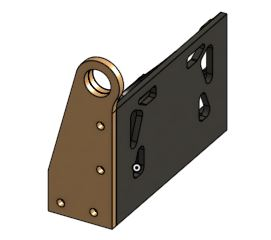
\includegraphics[width=0.95\textwidth]{Meetings/January/01-17-22/1-17-22_CAD_Figure1 - Nathan Forrer.JPG}
  \caption{Space for a REV bearing}
  \label{fig:011722_4}
\end{minipage}%
\hfill%
\begin{minipage}[b]{.48\textwidth}
  \centering
  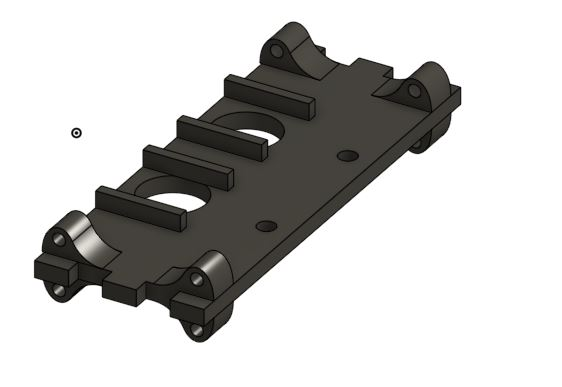
\includegraphics[width=0.95\textwidth]{Meetings/January/01-17-22/1-17-22_CAD_Figure2 - Nathan Forrer.JPG}
  \caption{Color sensor mounting points}
  \label{fig:011722_5}
\end{minipage}
\end{figure}

\begin{figure}[ht]
\centering
\begin{minipage}[b]{.48\textwidth}
  \centering
  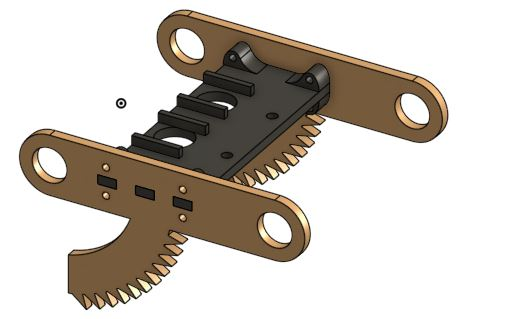
\includegraphics[width=0.95\textwidth]{Meetings/January/01-17-22/1-17-22_CAD_Figure3 - Nathan Forrer.JPG}
  \caption{Stopping arms}
  \label{fig:011722_6}
\end{minipage}%
\hfill%
\begin{minipage}[b]{.48\textwidth}
  \centering
  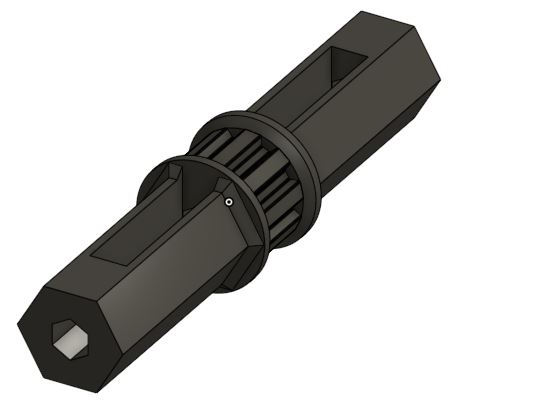
\includegraphics[width=0.95\textwidth]{Meetings/January/01-17-22/1-17-22_CAD_Figure4 - Nathan Forrer.JPG}
  \caption{The sweeper base}
  \label{fig:011722_7}
\end{minipage}
\end{figure}

\begin{figure}[htp]
\centering
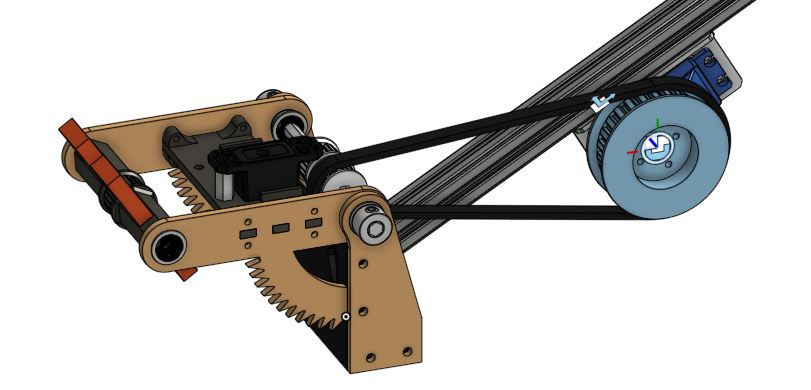
\includegraphics[width=0.95\textwidth, angle=0]{Meetings/January/01-17-22/1-17-22_CAD_Figure5 - Nathan Forrer.JPG}
\caption{The finished assembly}
\label{fig:011722_8}
\end{figure}



\whatsnext{
\begin{itemize}
    \item Print elements and Test them
    \item Cut and 3D print parts for new intake
    \item Test out new intake

\end{itemize} 
}

